%
% Homework or exam template 
% James A Miller (UAH Physics & Astronomy)
% 08/18/2015, 04/12/2023
%
% Uses the exam document class with some common math packages
%   and convenient custom macros.
% See exam class documentation for more question formats.
% Show answers by uncommenting the `\printanswers` statement after
%   `\begin{document}`.

%%%%%%%%%% PREAMBLE %%%%%%%%%%

\documentclass[11pt, addpoints]{exam}

% fonts
\usepackage{mathpazo}
\usepackage{helvet} % sans serif
\usepackage{courier} % mono
\usepackage[
    protrusion=true,
    activate={true,nocompatibility},
    final,
    tracking=true,
    kerning=true,
    spacing=true,
    factor=1100]{microtype}
\SetTracking{encoding={*}, shape=sc}{40}

% page setup
\usepackage[%
	paperwidth=8.5in, paperheight=11in,  
	left=1in, textwidth=6.5in, 
	top=1in, bottom=1in, 
	headsep=14pt, headheight=14pt, 
	footskip=10pt
	]{geometry}

% colors
\usepackage[svgnames, x11names, table]{xcolor}
\definecolor{plum}{rgb}{0.36078, 0.20784, 0.4}
\definecolor{chameleon}{rgb}{0.30588, 0.60392, 0.023529}
\definecolor{cornflower}{rgb}{0.12549, 0.29020, 0.52941}
\definecolor{scarlet}{rgb}{0.8, 0, 0}
\definecolor{brick}{rgb}{0.64314, 0, 0}
\definecolor{sunrise}{rgb}{0.80784, 0.36078, 0}
\definecolor{lightblue}{rgb}{0.15,0.35,0.75}

% hypertext
\usepackage[%
    colorlinks,%
    citecolor=plum,% color of links to references
    urlcolor=cornflower,% color of external links
    linkcolor=plum,% color of internal links
    breaklinks=true%
    ]{hyperref}

% math
\usepackage{amsmath}
\usepackage{mathtools}
\usepackage{xparse}
\usepackage{cases}
\usepackage{braket}
\usepackage[mleftright]{diffcoeff}
\usepackage{siunitx}
\usepackage{esvect} % for vectors with arrows (option for bold below)

% some useful macros
%     define \myqty
%     enclose math expression with autosized (), [], or {}.
%     For example, \myqty(\frac{1}{2})
\newcommand{\DeclareAutoPairedDelimiter}[3]{%
  \expandafter\DeclarePairedDelimiter\csname Auto\string#1\endcsname{#2}{#3}%
  \begingroup\edef\x{\endgroup
    \noexpand\DeclareRobustCommand{\noexpand#1}{%
      \expandafter\noexpand\csname Auto\string#1\endcsname*}}%
  \x}
\DeclareAutoPairedDelimiter{\pqty}{(}{)} % paren quantity
\DeclareAutoPairedDelimiter{\bqty}{[}{]} % bracket quantity
\DeclareAutoPairedDelimiter{\absqty}{|}{|} % brace quantity
\NewDocumentCommand\myqty{ d() d[] d|| }%
{%
    \IfNoValueTF{#1}%
      { \IfNoValueTF{#2}{\absqty{#3}}{\bqty{#2}} }%
      { \pqty{#1} }%
}%

%     define bold vectors
%     Use star * for Greek and italic Roman
\DeclareDocumentCommand\vectorbold{ s m }{\IfBooleanTF{#1}{\boldsymbol{#2}}{\mathbf{#2}}} 
\DeclareDocumentCommand\vb{}{\vectorbold} % Shorthand

%     define bold unit vectors
%     Use star * for Greek and italic Roman
\DeclareDocumentCommand\vectorunit{ s m }{\IfBooleanTF{#1}{\boldsymbol{\hat{#2}}}{\mathbf{\hat{#2}}}} 
\DeclareDocumentCommand\vu{}{\vectorunit} % Shorthand 

% graphics
\usepackage{graphicx}
\usepackage[%
    font=small, 
    margin=10pt, 
    labelfont=bf, 
    labelsep=endash, 
    justification=raggedright
    ]{caption}
 
% header and footer
\usepackage{lastpage}
\pagestyle{headandfoot}
\runningheadrule
\newcommand{\continuedmessage}{%
	\ifcontinuation{\footnotesize Question \ContinuedQuestion\ continues\ldots}{}
 }
\runningheader{PH 652}%
	{Homework Assignment}%
	{Page \thepage\ of \pageref{LastPage}}
\runningfootrule
\footer{Name:}%
	{}%
	{
	\ifincomplete{Question \IncompleteQuestion\ continues on the next page\ldots}
	{\iflastpage{End of assignment}{Please go on to the next page\ldots}}
	}

% points for questions
\pointsinrightmargin
\pointsdroppedatright
\marginpointname{ \points}
\pointformat{\boldmath\themarginpoints}
\bracketedpoints

% for true/false questions
\newcommand{\tf}[1][{}]{%
    \fillin[#1][0.25in]% 
    }

%%%%%%%%%% DOCUMENT %%%%%%%%%%

\begin{document}

% comment out to hide answers
%\printanswers

\thispagestyle{empty}

Name:\rule{.5\textwidth}{1pt}\par
\vspace{0.2in}

\noindent
\begin{minipage}[t]{\textwidth}%
	\centering
	%\includegraphics[width=1cm]{logo} \par
	The University of Alabama in Huntsville\par
	Course number \quad Course title \par
	\underline{Homework Assignment/Exam XX} \par
\end{minipage}

\begin{center}
  \fbox{\fbox{\parbox{5.5in}{\centering
        Turn in this assignment page on top of your solutions. Solutions must be neat and readable. No credit for anything that is not. Clearly indicate your final answers.
        }}}
\end{center}
\vspace{0.2in}

\begin{center}
  \gradetable[h][questions]
\end{center}
\vspace{0.2in}

%%%%%%%%%% QUESTIONS %%%%%%%%%%

\begin{questions}

%------------ Question with parts ---------------------------------------
\question \label{ques:questionparts}
This is a question with multiple parts. Add or subract as needed. Of course, questions and solutions can have math formulae. Solutions are printed if \textsf{$\backslash$printanswers} is uncommented after the beginning of the document.

\begin{parts}
\part[5]\label{ques:parta} The first part of the question.
\droppoints

\part[15]\label{ques:partb} The second part.
\droppoints

\part[5]\label{ques:partc} The third part. Add or subtract parts as needed.
\droppoints
\end{parts}
\droptotalpoints


\begin{solution}
The solution goes here.
\begin{parts}
\part The solution goes here.

\part The solution goes here.

\part The solution goes here.
\end{parts}
\end{solution}
% --------------------------------------------------------------------------


%------------ Question with no parts ------------------------------------------
\question[5] \label{ques:questionnoparts}
This is a question with no parts.
\droppoints

\begin{solution}
Solution to the question with no parts.
\end{solution}
% --------------------------------------------------------------------------


%------------ Question with multiple choice ----------------------------------
\question[10] \label{ques:questionmc}
There are many question formats we can use. Here is a multiple choice. The correct answer is noted in the options, and will be printed when the solutions are enabled. Here's the question: What is Newton's Second Law?

\begin{choices}
\correctchoice $\vb{F} = m \vb{a}$
\choice $S = k_\text{B} \ln\Omega$
\choice $p_x = (\hbar/i) \partial_x$
\choice $v_x = \difs xt$
\end{choices}
\droppoints
% --------------------------------------------------------------------------


%------------ Question with multiple choice and checkboxes -------------------
\question[10] \label{ques:questionmcbox}
This is a multiple choice question with checkboxes. What is Newton's Second Law?

\begin{checkboxes}
\correctchoice $\vb{F} = m \vb{a}$
\choice $S = k_\text{B} \ln\Omega$
\choice $p_x = (\hbar/i) \partial_x$
\choice $v_x = \difs xt$
\end{checkboxes}
\droppoints
% --------------------------------------------------------------------------


%------- Question with multiple choice and checkboxes in one line ----------
\question[10] \label{ques:questionmclinebox}
This is a multiple choice question with checkboxes, but the choices all one line to save space. The correct choice will print when answers is enabled in the preamble. What is Newton's Second Law?

\begin{oneparcheckboxes}
\correctchoice $\vb{F} = m \vb{a}$
\choice $S = k_\text{B} \ln\Omega$
\choice $p_x = (\hbar/i) \partial_x$
\choice $v_x = \difs xt$
\end{oneparcheckboxes}
\droppoints
% --------------------------------------------------------------------------


%------------ Question with fill in the blank -------------------
\question[10] \label{ques:questionfillin}
This is a fill in the blank question. Again, the answer is noted in the question. Here's the question: 
The next total solar eclipse visible in the US is in the month of \fillin[April].
\droppoints
% --------------------------------------------------------------------------


%------------ Question true/false -------------------
\question[10] \label{ques:questiontf}
\tf[T] This is true/false question. The world is not enough.
\droppoints
% --------------------------------------------------------------------------


%------------ Question with a figure -------------------
\question[10] \label{ques:questionfig}
This is a question with a figure.

    \begin{minipage}[t]{\linewidth}
        \centering
        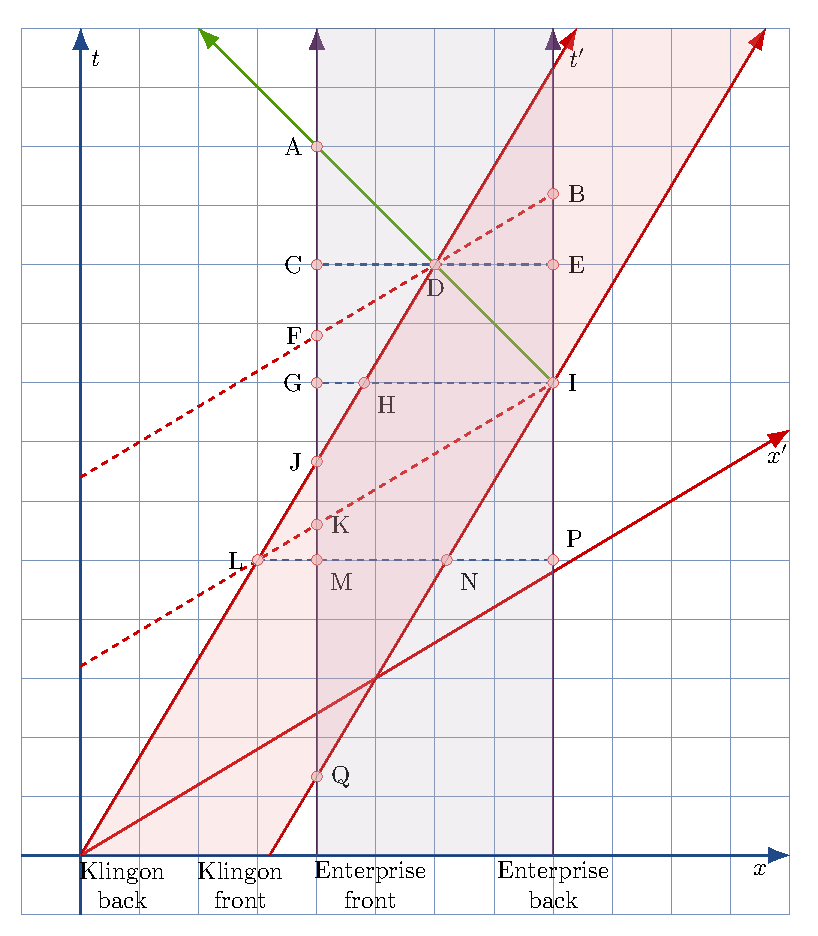
\includegraphics[scale=0.5]{fig.pdf}
        \captionof{figure}{This is a figure caption.}
    \end{minipage}
    
\begin{parts}
\part[5]\label{ques:partaf} The first part of the question.
\droppoints

\part[15]\label{ques:partbf} The second part.
\droppoints

\part[5]\label{ques:partcf} The third part. Add or subtract parts as needed.
\droppoints
\end{parts}
\droptotalpoints


\begin{solution}
The solution goes here.
\begin{parts}
\part The solution goes here.

\part The solution goes here.

\part The solution goes here.
\end{parts}
\end{solution}
% --------------------------------------------------------------------------


 
\end{questions}

%%%%%%%%%% END QUESTIONS %%%%%%%%%%

\begin{center}
\rule{.5\textwidth}{1pt}
\end{center}

\end{document}